%\todo[inline]{existing game research?? own section?}

\section{Games and the Virtual Reality}
\label{sec:gamesNvr}

To catch a brief insight into games that both support playing with or without HMD and to further introduce research aspects of the following section this paragraph is intended to list a few differences, similarities and uniqueness within games. An overview of these games can be found in \textbf{Table~\ref{tab:popularGames}}, where some properties of them are listed. 

Starting with \textit{Minecraft}. an open world sandbox game where the player controls his playable character by navigating with the keyboard or game controller. The goal is to mine blocks of different material and craft them into objects which he will need to complete the game. As it is an open world game the player can move to different areas in order to gather some items needed. 

A disadvantage of this game in VR is the locomotion method needed in order to move around the world. Since the game has not many stationary tasks and it depends on the ability of the user to move around it holds greater potential for the virtual reality sickness occurring.

\begin{figure}
	\centering
	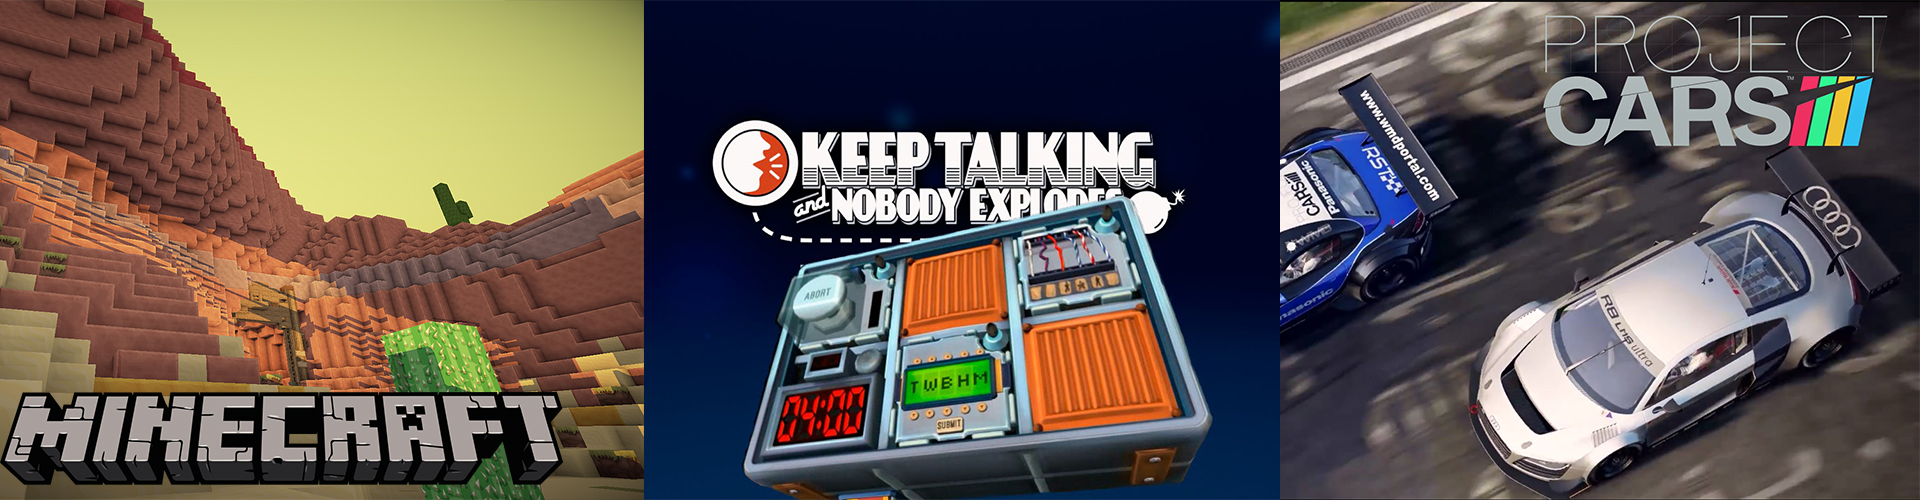
\includegraphics[width=0.99\columnwidth]{./figures/banner}
	\caption[banner]{The three presented games. FLTR Minecraft, Keep talking and nobody explodes and Project CARS. Each game offers native VR Support on multiple devices and has different interaction methods for locomotion.\footnotemark}~\label{fig:banner}
\end{figure}
\footnotetext{
	\textcopyright~Mohjang, Steel Crate Games, Slightly Mad Studios, [Online; accessed January 04., 2017],[Digitally edited] \url{https://pixabay.com/p-354458} \url{https://i.ytimg.com/vi/Apwa_ksMvM0/maxresdefault.jpg} \url{https://i.ytimg.com/vi/RggvBJ2ANWo/maxresdefault.jpg} \ccbyncsa
}

Another game is \textit{Keep Talking and Nobody Explodes} a puzzle game where one player has to describe and disarm a virtual explosive charge in a given time. His team members, who cannot see the bomb, have to explain what he has to do in order to disarm the bomb and to save his and the team members lives. The game mechanics are different from those of Minecraft. The player wearing the HMD has a stationary task and just needs to interact with objects in his direct vicinity. 

Because of this only natural locomotion the peril of becoming sick is very weakly present.

\textit{Project CARS} is a racing simulation for Microsoft Windows, PlayStation 
4, and Xbox One. It offers standard racing simulation whilst also providing the 
kind of advanced features usually reserved for PC-only simulators.

The locomotion is solely a cockpit locomotion, meaning that the player is 
sitting in a virtual car and steering with different interfaces. Because of the 
visual stimuli of moving inside a car but neither the vibration nor the 
acceleration is palpable the user is weakly prone to becoming VR sick.

In VR these games offer an immerse way to include the gamer into the game. 
Because of the different approaches to solving problems of VR more static games 
like \textit{Keep Talking and Nobody Explodes} and \textit{Project CARS} have 
greater potential in becoming very popular in the VR gaming community. 

There are no numbers available regarding the players per month that are using 
VR for their gaming experience in these games. 

%\blindtext[1]

\begin{table}%[h]
	\caption{Popular games played in late 2016. The games offer a regular play mode, using the monitor, and a VR play mode with both the Oculus Rift and the HTC Vive}~\label{tab:popularGames}
	
	%{}\fontfamily{pcr}\selectfont
	\renewcommand{\arraystretch}{1.3}% for the vertical padding
	\begin{tabular*}{\columnwidth}{ p{33mm} l r l }
		Gametitle & Genre & \parbox[c][2.2em][t]{2cm}{\begin{flushright}$\dfrac{Players}{Month}$(\footnotemark)\end{flushright}} & LM\footnotemark \\
		\hline
		Minecraft & RPG\footnotemark & 990 K & ALM \\
		Keep Talking and \newline Nobody Explodes & Puzzle & 153.3 & NLM \\
		Project CARS & Racing & 1.01 K & CLM\\
	\end{tabular*}
	%}
	
\end{table}

\footnotetext[3]{\url{http://steamcharts.com}, accessed Jan. 3., 2017}
\footnotetext[4]{Types of Locomotion (LM): Natural Locomotion (NLM), Cockpit Locomotion (CLM), Artificial Locomotion (ALM) See also: Section\ref{sec:exLocomotion}:~Locomotion}
\footnotetext[5]{RPG: Role-Playing Game}
%\todo[inline]{Die footnotes werden nicht richtig nummeriert... von hand fixen bei submission!?}

\subsection{Popularity Of VR Games}
Since the beginning of game development and virtual reality in the 20th century 
there has been a huge potential to include the user in a virtual environment. 
Some systems have been developed in the past five years that simplify some 
processes of work for different disciplines. 

Games have just lately adopted the potential for this immerse form of gaming. VR offers new dimensions of freedom to include the player into a game world and to tell stunning stories.

Using a virtual environment to show worlds to players has the great advantage of giving them the feeling of being in the middle of the event, but the game has very limited possibilities to tell stories with much variety. This is that the game can not change perspectives as easy. 

While games that do not use VR can handle attention themselves by just moving the camera VR is bound to the camera perspective of the gamer. These games can show views from other perspectives without worrying about the user becoming confused. VR-Games need another way to handle interaction, the user has to hold some kind of controller interface to tell the system what he wants to do. Games outside of VR have similar interface problems but the process has been researched more than the interaction with VR-Games. Simultaneously VR games require a much more active way of interaction, because the user has to complete physical tasks as he is playing the game. This can be a negative point for people who would just rather enjoy a game than have a minor workout while playing.

A study realized in January 2017 by myself spanning over 40 participants showed that a majority of people had never played a virtual reality game before. It was found that most persons describing themselves as gamers would agree that VR games should be immersive and intuitive. Intuitive meaning that the interaction and locomotion in the game is as close as possible to movement in the real world.

The study has also shown that most of the people that have tried a VR game in person would describe themselves as gamers, although also many other participants affirmed this question. The question resulting is if people are more likely to test vr in person if they think they already are gamers.

\begin{table}[h]
	\caption{Gamers and non games have been asked to rate the following aspects, whereas 1 means they strongly disagree, 4 means they strongly agree - 0: unsure. The question asked was whether they thing a VR game should be...}~\label{tab:study}
	
	\renewcommand{\arraystretch}{1.3}% for the vertical padding
	\begin{tabular*}{\columnwidth}{l @{\extracolsep{\stretch{1}}}*{5}{r}@{}}
		 & 1 & 2 & 3 & 4 & 0 \\
		\hline
		Innersive & 0 & 0 & 10 & 34 & 2 \\
		Active & 2 & 10 & 21 & 1 & 2 \\
		Intuitive & 0 & 2 & 24 & 16 & 4 \\
		Simple & 4 & 24 & 9 & 4 & 5 \\
	\end{tabular*}
	
\end{table}

\begin{figure}[h]
	\centering
	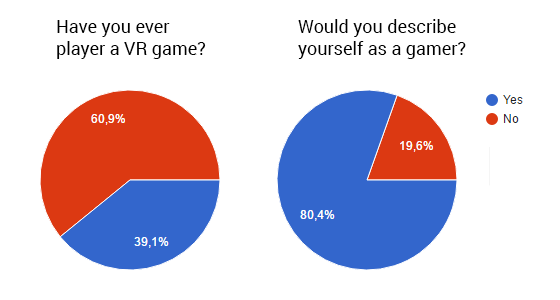
\includegraphics[width=0.99\columnwidth]{./figures/study}
	\caption[study]{Most of the people asked have not tried any VR games yet. Also most of the participants would say they are gamers.}~\label{fig:study}
\end{figure}

\subsection{Motivation In Games}

The people of \textit{Quantic Foundry} have developed an online survey for categorizing 
gamers and their motivation. By filling in the survey in an 
online app users could receive a report on their gaming motivation. They have been using a bootstrap approach to collect data and iterate on the model. While the 
data came in they kept rerunning a factor analysis until a robust model 
emerged. 

This resulted in 220.000 people who took the test and received their 
personalized results online. Among the people who took the survey where 81\% 
male and 18\% female users. The age ranged from 13 to 77 years and the median 
was 25 years. Most of the gamers came from north America and the western EU.

The Model that emerged from the data they have got can be seen in 
\textbf{Figure~\ref{fig:gameMotivation}}~\footnotemark[6] and the clustered 
categories are described as follows:

\begin{figure}
	\centering
	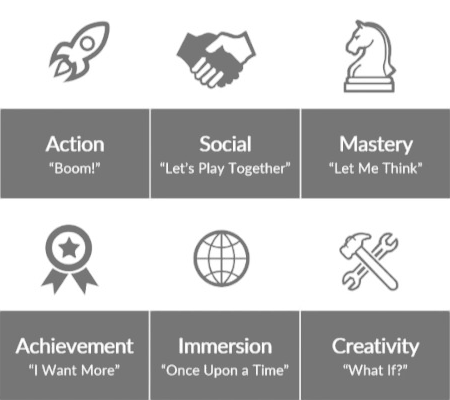
\includegraphics[width=0.99\columnwidth]{./figures/motivation}
	\caption[motivation]{The 6 categories of motivation in games. 
	\footnotemark[6]}~\label{fig:gameMotivation}
\end{figure}

\begin{description}%[align=right,labelwidth=2.5cm]
	\item[Action] \textit{The appeal of mayhem and chaos and exciting, fast 
	paced game play context. Action as motivation addresses people who like the 
	thrill and the challenge.}
	\item[Social] \textit{Contains both; the challenge and the interesting 
	collaboration and socializing. The social category describes people who 
	like to be together with others, socialize, help and/or compete with 
	others.}
	\item[Mastery] \textit{Is about long term planning and thinking. Whether it 
	is practicing the game to take on the highest difficulty or the enjoyment 
	of strategy; thinking and planning ahead. It mostly appeals to people 
	making complex decisions.}
	\item[Achievement] \textit{Different ways of getting points in the context 
	of the game. On one side points as in points, stars, trophies et cetera, or 
	points in the sense of power: leveling up as quickly as possible, getting 
	the best equipment and gear.}
	\item[Immersion] \textit{Different ways of becoming embedded in the story 
	of the world. The sheer sense of being immersed, being someone else, 
	somewhere else. Engaging with an elaborate plot, interesting characters and 
	deep back stories.}
	\item[Creativity] \textit{The appeal of making the game your own in any 
	kind of way. Creating a unique avatar, customizing your city. And on the 
	other hand discovery. Playing the game in the broadest sense of the word.}
\end{description}
\footnotetext[6]{"Gamer Motivation Profile Findings - \#GamesUR US Conference 2016" Quantic Foundry Website, March, 25., 2015, accessed November 05., 2016, \url{http://quanticfoundry.com/2016/04/07/gdc-talk/}}

At a high level there are three motivational clusters that emerge from this 
structure. These clusters can be seen in 
\textbf{Figure~\ref{fig:motivationClusters}}

The first is the action-social cluster, combining the action gameplay with 
social activities in games by more fine grain categories such as 
\textit{community}, \textit{destruction}, \textit{excitement} and so forth. 

The second cluster is mastery-achievement, where players want to become better. 
In this category points like \textit{competition}, \textit{strategy} and 
\textit{challenge} are to be found. 

And the last cluster is the immersion-creativity one. With points like 
\textit{story}, \textit{fantasy} and \textit{design} this cluster is the most 
compact in its variance. 

Interesting is that there are two traits which form kind of like a bridge 
between clusters. For one that is \textit{discovery}, where the player wants to 
discover new ways of playing the game as well as discover exciting places 
inside of the in game world. The second bridge is \textit{power} where the user 
can satisfy the urge to master the game and also be in the action-social 
cluster with mayhem et cetera. 

To draw a bow over to the virtual reality aspect of gamer motivation it is 
important to notice that not all motivational categories convey easily to the 
VR aspect. While \textit{immersion} and \textit{creativity} are already well 
implemented in todays games missing research on the \textit{social} and 
\textit{mastery} motivations avert a pivotal statement on the subject. 

In VR games today not many approaches have been made to include other real 
players into the game. A very small fraction of games has a well developed idea 
of how to include a 'Player 2' into the game and even less games have a perfect 
representation of another player in the game, i.e. via avatar. 

For a VR game it is apparent that the immersion is highly given, sadly there 
has not been made a lot of research on the impact towards people and a clear 
answer can not be given when asked what affects it has on the human psychology. 

\begin{figure}
	\centering
	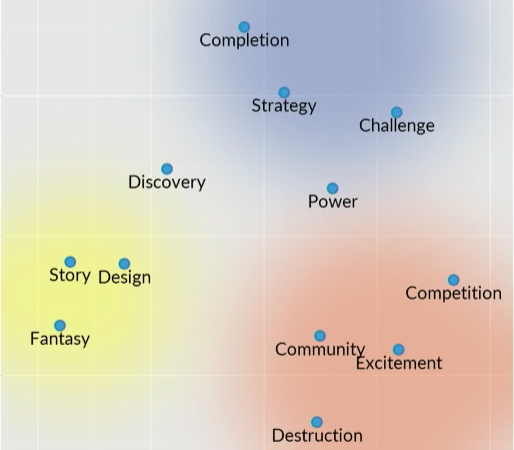
\includegraphics[width=0.99\columnwidth]{./figures/clusters}
	\caption[motivation]{Three motivational clusters. Blue is 
	mastery-achievement cluster, yellow is immersion-creativity cluster and red 
	is action-social cluster.~\footnotemark[6]}~\label{fig:motivationClusters}
\end{figure}

\subsection{Input Techniques}
Because many of the HMD of earlier sections use similar approaches to enable 
the user to interact with the game this paragraph is only to show some 
similarities in these. 

Users can often interact with the game via interface devices such as mouse and 
keyboard, game controller oder steering wheels. For HMD like the 
\textit{Samsung Gear VR} and the \textit{Daydream View} no generic 
interfaces are existent. The \textit{Samsung Gear VR} can be extended via gamepad 
to form a better experience the simplifies interaction with the virtual 
environments. The \textit{Daydream View} supports an remote control device 
similar to a gamepad but has less interaction possibilities that other devices.

All the other devices have bundled interaction possibilities to perform even 
complicated maneuvers in VR. 

From past developments such as the \textit{XBox Kinect} motion tracking was established, using cameras. Nowadays many other approaches are available so that the detection of body parts is not only a visual problem anymore. It was shown that other forms of interaction provide direct feedback to the base system and fit these problems better at these times. To free the users from bulky interfaces the motion tracking with cameras remains a prosperous candidate.

In the following section \textbf{Further Research Trends} some improvements for 
the interaction with HMD will be discussed.

\subsection{Existing Locomotion Techniques}
\label{sec:exLocomotion}

There are three basic categories of locomotion present at this time in VR: 
\textbf{artificial}, \textbf{natural} and \textbf{cockpit locomotion}.

The principle described as \textit{artificial locomotion} is the method of 
moving in the virtual environment by triggering interfaces and telling the game 
where you want to go. This method is often used because it offers a great 
degree of freedom. But it also has the greatest disadvantage because the users 
senses provide different signals to the brain and thus holds the greatest 
potential to cause motion sickness.

There are different specific methods of artificial locomotion:
\begin{description}
	\item[Interface movement]By using the provided interface devices the user 
	can steer the virtual representation of himself in different directions. 
	Depending on the game it has up to three dimensions of motion and thus 
	degrees of freedom.
	\item[Point and teleport]The user has to point, using his provided input 
	method, as described before, on a surface and confirm the selection. The 
	game then moves the camera, the virtual representation of the player to the 
	location. By using this method the user can move through a world without 
	the need to actual physical change of location. An advantage is that 
	the user can observe at worlds from different points of view.
\end{description}

In \textit{natural locomotion} only the motion and rotation of the users head 
is used, no movement through an input interface. This interaction with the game 
wolds is very static and thus these kind of games do not cause sickness and 
enable constant mental presence and longer playtimes to the user.

With natural locomotion the user is limited to a local position in the game as 
well as the virtual environment. But there are also different approaches to 
make games using this 
\begin{description}
	\item[Interaction with objects]The user can interact with objects right in 
	front and around him. The objects are movable, turnable and sometimes 
	scalable by using the game interfaces.
	\item[Moving the view around the main game object]In the game the user can 
	specify from what angle he wants to look at the game objects in focus. 
	Again by using the game interface he can position the camera and with that 
	the position from which he is interacting with the object.
\end{description}

\textit{Cockpit locomotion} games use a vehicle with a cockpit to let you traverse a large environment. Whether this makes you sick varies between person, the size of the cockpit, and the intensity of the maneuvers that you are pulling. Generally, you will not get sick if you are only gently moving around in these games. 

In cockpit locomotion the movement of the camera is not possible without moving 
the surrounding environment
\begin{description}
	\item[Cockpit]With a near vicinity of objects displaying a cockpit, such as 
	the one of an airplane, a car or comparable vehicles the user can move 
	himself and his surrounding around the virtual game world and with this 
	move from one place to another.
	\item[Stationary Items]Meaning surroundings that are not movable. In this 
	locomotion technique only the orientation of the device the user is using 
	can be changed. This can be adapted to stationary weaponry or other 
	stationary items.
\end{description}

In research are not many approaches to the pros and cons of these locomotion 
techniques and no clear statement can be given on the best solution. 
Future research trends will be looked at in the following section under 
\textbf{Locomotion}
